% set \papertrue when printing to paper

\newif\ifpaper
% \papertrue
\paperfalse
\ifpaper
\PassOptionsToClass{handout}{beamer}
\fi

%%%%%%%%%%%%%%%%%%%%%%%%%%%%%%%%%%%%%%%%%%%%%%%%%%%%%%%%%%%%%%%%%%%%%%%%%%%%%%%%

\documentclass{beamer}
\usepackage[T1]{fontenc}
\usepackage{arev}
\usepackage{textcomp}
\usepackage{ragged2e}
\usepackage{tikz}
\usepackage{hyperref}
\usetikzlibrary{positioning}
\usepackage{amsmath}
%%%%%%%%%%%%%%%%%%%%%%%%%%%%%%%%%%%%%%%%%%%%%%%%%%%%%%%%%%%%%%%%%%%%%%%%%%%%%%%%

\author{ Antony Cervone and Luca Formaggia}
\title{An too long introduction to git}
\date{2015 V2}
\pgfdeclareimage[width=0.8\textwidth]{gitdict}{figures/dict.pdf}
\titlegraphic{\pgfuseimage{gitdict}}

%%%%%%%%%%%%%%%%%%%%%%%%%%%%%%%%%%%%%%%%%%%%%%%%%%%%%%%%%%%%%%%%%%%%%%%%%%%%%%%%

\usefonttheme{professionalfonts}
\setbeamertemplate{navigation symbols}{}
\setbeamercolor{shell}{fg=black,bg=black!20}
\setbeamercolor{separation line}{use=structure,bg=structure.fg}

%%%%%%%%%%%%%%%%%%%%%%%%%%%%%%%%%%%%%%%%%%%%%%%%%%%%%%%%%%%%%%%%%%%%%%%%%%%%%%%%

% make _ (underscore) a common character (math does not work here!)
\makeatletter
\catcode`\_=12

\newenvironment{shell}{%
\footnotesize\flushleft\hrule height 0.1ex
\tt\begin{beamercolorbox}[sep=1ex,left]{shell}%
}{%
\end{beamercolorbox}
\hrule height 0.1ex
\endflushleft\par
}

%%%%%%%%%%%%%%%%%%%%%%%%%%%%%%%%%%%%%%%%%%%%%%%%%%%%%%%%%%%%%%%%%%%%%%%%%%%%%%%%

\newcommand*{\tshell}[1]{{\usebeamercolor[fg]{shell}\colorbox{bg}{\tt#1}}}

\newcommand*{\psone}[1][ant]{\$>~}
\newcommand*{\nl}{\textbackslash\\>~}
\newcommand*{\var}[1]{{\it<#1>}}

\newcommand*{\boxltr}[1]{
{\usebeamercolor[fg]{frametitle}
\tikz[remember picture,baseline=(t@mp.base),minimum width=3ex,minimum height=3ex] 
\node [fill=bg,draw=fg,thick] (t@mp) {#1};}
}

%%%%%%%%%%%%%%%%%%%%%%%%%%%%%%%%%%%%%%%%%%%%%%%%%%%%%%%%%%%%%%%%%%%%%%%%%%%%%%%%

\setbeamertemplate{title page}
{
\vfill
\begin{centering}
\titleline
{\usebeamercolor[fg]{titlegraphic}\inserttitlegraphic\par}
\vspace{-12pt}\titleline
\begin{beamercolorbox}[sep=8pt,center]{title}
\usebeamerfont{title}%
\inserttitle
\par%
\end{beamercolorbox}%
\begin{beamercolorbox}[sep=8pt,center]{author}
\usebeamerfont{author}\insertauthor
\end{beamercolorbox}
\begin{beamercolorbox}[sep=8pt,center]{date}
\usebeamerfont{date}\insertdate
\end{beamercolorbox}\vskip0.5em
\end{centering}
\vfill
\Tiny{Merriam-Webster's Collegiate Dictionary, p.529}
}

%%%%%%%%%%%%%%%%%%%%%%%%%%%%%%%%%%%%%%%%%%%%%%%%%%%%%%%%%%%%%%%%%%%%%%%%%%%%%%%%

\ifpaper % printing to paper

\usepackage{pgfpages}
\pgfpagesuselayout{2 on 1}[a4paper,border shrink=0mm]

\fi

%%%%%%%%%%%%%%%%%%%%%%%%%%%%%%%%%%%%%%%%%%%%%%%%%%%%%%%%%%%%%%%%%%%%%%%%%%%%%%%%

\usecolortheme[named=black]{structure}

\newcommand{\titleline}[1][0.025cm]{%
\begin{beamercolorbox}[wd=\paperwidth,ht=#1,center]{separation line}%
\end{beamercolorbox}%
}

\setbeamertemplate{headline}
{%
\Large
\vskip1ex%
\ifnum \thepage>1%
\titleline
\else%
\begin{beamercolorbox}[wd=\paperwidth,ht=0.025cm,center]{structure}%
\end{beamercolorbox}
\fi
}
\addtobeamertemplate{frametitle}{}{\fontsize{10}{7.5}\selectfont \titleline}

\makeatother

\begin{document}


%%%%%%%%%%%%%%%%%%%%%%%%%%%%%%%%%%%%%%%%%%%%%%%%%
\begin{frame}
\titlepage
\end{frame}
%%%%%%%%%%%%%%%%%%%%%%%%%%%%%%%%%%%%%%%%%%%%%%%%%
\begin{frame}{What is a revision control system (RCS)}
\titleline
{\small
  Software needs to be \textcolor{blue}{maintained},
 \textcolor{blue}{debugged}, \textcolor{blue}{improved}...
while keeping track of the changes and being able to recover old revisions
if needed.
\smallskip

Those task can be done automatically using a \textcolor{red}{Revision Control System}.
\smallskip

In addition, one may want to keep a copy of the code (and of all its changes) in a remote repository, for safety and for sharing with others.

\smallskip

Most common RCS: CVS, RCS, git, mercurial (Hg)....
}
\titleline
\end{frame}

\begin{frame}{Centralised vs Distributed RCS}
\begin{minipage}{0.45\textwidth}
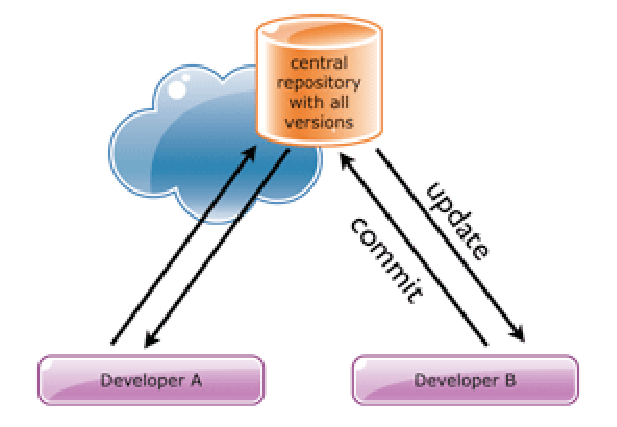
\includegraphics[width=0.98\textwidth]{figures/centralised}
\end{minipage}
\hfill
\begin{minipage}{0.45\textwidth}
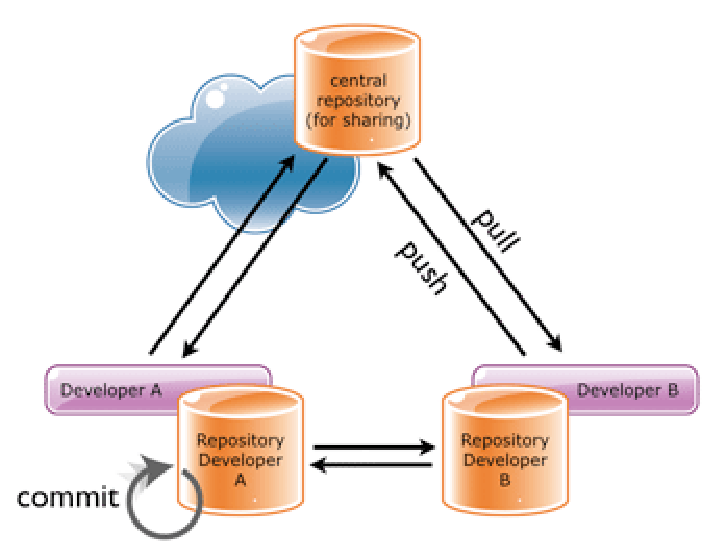
\includegraphics[width=0.98\textwidth]{figures/distributed}
\end{minipage}
\medskip

Centralised RCS compares with a distributed RCS as an \textcolor{blue}{hub} compares with a \textcolor{blue}{peer--to--peer} model.
\end{frame}
\begin{frame}{The philosophy of a distributed RCS}
\begin{itemize}
\item Each user has a local copy of the repository: you have full control of all the history even if you are not connected to the web
\item Most commands operate on the local copy (minimize communications).
\item You may have multiple remote repositories: better distributed development.
\end{itemize}
\end{frame}
\begin{frame}{A Distributed RCS: git}
\titleline
{%
\small
\RaggedRight
Git is a distributed revision control system with an emphasis on speed.
Git was initially designed and developed by Linus Torvalds for Linux kernel
development. 

\alert{Every Git working directory is a full-fledged repository
with complete history and full revision tracking capabilities, not dependent on
network access or a central server.}
}%
\titleline

In git (almost) every command operated just on the  \textcolor{red}{local}
repository. Indeed \textcolor{blue}{you do not even need a remote repository to use git!}.
\end{frame}
% %%%%%%%%%%%%%%%%%%%%%%%%%%%%%%%%%%%%%%%%%%%%%%%%%
% \begin{frame}{A graphic approach}
% \begin{center}
% 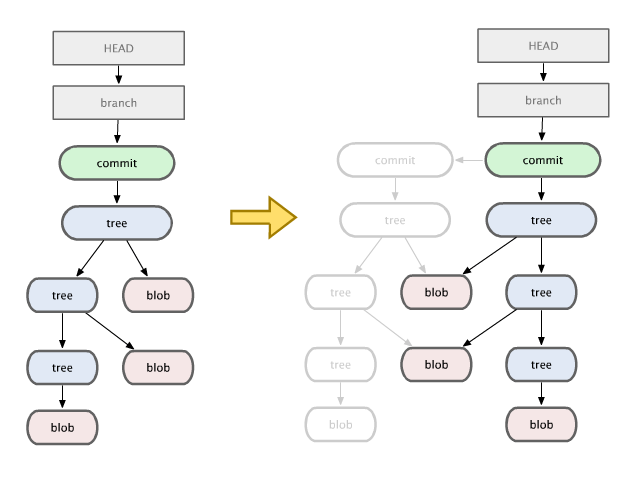
\includegraphics[width=.8\textwidth]{figures/git_trees}
% \end{center}
% \end{frame}
%%%%%%%%%%%%%%%%%%%%%%%%%%%%%%%%%%%%%%%%%%%%%%%%%
\begin{frame}{The only commands that communicate with a remote repository}
Even if you do not yet know what they do, here there are the (only) three commands used by git to operate on a remote repository:
\medskip

\begin{center}
\alert{push, fetch, pull}
\end{center}
\end{frame}

\begin{frame}{First thing to do}
\titleline
If you have never used git on a computer you should first let git know who you are (so that people can blame you for your wrong deeds or cherish you for your programming skill!)

\begin{shell}
git config --global user.name ``Luca Formaggia''
\end{shell}
\begin{shell}
git config --global user.email ``micky.mouse@gmail.com''
\end{shell}

\texttt{git config} tells git to change some git configuration. 

\texttt{global} makes it to change some global parameter,
i.e. a parameter that applies to all yours git working directories in
that computer.  \titleline
\end{frame}

\begin{frame}{Need help?}
\titleline

Git has an integrated help. If you need help for the command \texttt{command}
just do

\begin{shell}
git help command 
\end{shell}

Git uses a lot of terms that may confuse you at the beginning (and not only at the beginning...). A useful command is 

\begin{shell}
git help glossary
\end{shell}

You find more on the \href{http://git-scm.com/book}{Git Book} (git-scm.com/book)
\titleline
\end{frame}
\begin{frame}{More help?}
Other useful commands
\begin{shell}
git help tutorial
\end{shell}
A tutorial
\begin{shell}
git help tutorial-2
\end{shell}
The second part of the tutorial.
\end{frame}


\begin{frame}{Create/clone a repo}
A local repository. In the directory where you want to create it:
\begin{shell}
\psone git init
\end{shell}
Cloning from an existing remote repo
\begin{shell}
\psone git clone \nl \var{username}@cmcsforge.epfl.ch:/gitroot/lifev/lifev
\end{shell}
From a  mox repository
\begin{shell}
\psone git clone gitolite@gitserver.mate.polimi.it:eni-lifev
\end{shell}
\end{frame}

\begin{frame}{Github}
\href{https://github.com/}{Github} (github.com) is a site that allows you to create repositories and shere them with others. It provides also a nice web interface. 

\textcolor{red}{We will use github for the examples of the PACS course}. 

\end{frame}
%%%%%%%%%%%%%%%%%%%%%%%%%%%%%%%%%%%%%%%%%%%%%%%%%
%\begin{frame}{Protocols for connection to remotes}
%\begin{center}
%\begin{tabular}{ccccc}
%PROTOCOL      & PORT & READ & WRITE & PUBLIC \\
%\hline \\
%\tshell{ssh}  & 22   & YES  & YES   & NO     \\
%\tshell{git}  & 9418 & YES  & YES   & YES/NO \\
%\tshell{http} & 80   & YES  & NO    & YES    \\
%\end{tabular}
%
%\vspace{1cm}
%not exclusive! You may even send repository changes via mail or using a USB stick! 
%\end{center}
%\end{frame}
%%%%%%%%%%%%%%%%%%%%%%%%%%%%%%%%%%%%%%%%%%%%%%%%%
\begin{frame}{Edit!}
modify the files in the repo
\begin{shell}
\psone edit the sources \ldots \\
\end{shell}
show status of the repo
\begin{shell}
\psone git status \\
\tiny%
\# On branch \var{branch_name} \\
\# Changes to be committed: \\
\#   (use "git reset HEAD <file>..." to unstage) \\
\# \\
\#       modified:   file1.cpp \\
\# \\
\# Changed but not updated: \\
\#   (use "git add <file>..." to update what will be committed) \\
\#   (use "git checkout -- <file>..." to discard changes in working directory) \\
\# \\
\#       modified:   file2.cpp \\
\# \\
\# Untracked files: \\
\#   (use "git add <file>..." to include in what will be committed) \\
\# \\
\#       file3.cpp \\
\end{shell}
\end{frame}
\begin{frame}{The possible state of a file in the working directory}
\begin{itemize}
\item \alert{untracked} The file is not under git control. Maybe is just a temporary file. Or you want to put it under control using \texttt{git add}.
\item \alert{modified} The file has been modified since the last \textcolor{blue}{commit} in the repository. May be you want \texttt{add} it to the staging area.
\item \alert{staged} (in the index). Ready to be committed in the repository with a \texttt{git commit}
\end{itemize}
{\small
Beware: when you run \texttt{git add filename} to a modified file you put 
a snapshot of that file in the staging area. If you modify it again before the commit you need to do \texttt{git add} again (unless you want to commit the previous version).
}
\end{frame}

%%%%%%%%%%%%%%%%%%%%%%%%%%%%%%%%%%%%%%%%%%%%%%%%%
\begin{frame}{Commit}
show differences with the last commit
\begin{shell}
\psone git diff \var{branch} \var{files}
\end{shell}
stage files for a commit
\begin{shell}
\psone git add \var{edited_files}
\end{shell}
create a new commit in the repository
\begin{shell}
\psone git commit \\
\ldots \\
<vim editor will come up,\\ write a description for the commit>
\end{shell}
\begin{shell}
\psone git commit -m "message"\\
\end{shell}
The last command writes the commit message directly.
\end{frame}
\begin{frame}{What to put in a commit message}
\titleline
\begin{shell}
A first line with a brief description (it is the one that is shown by some
git commands)\\
\vspace{0.3cm}

Possibly followed by an empty line and a detailed description (possibly wrap lines to 72 characters)\\
\vspace{0.3cm}
 
Paragraphs are separated by empty lines.\\
\vspace{0.3cm}
 
- you may use lists using the - character
\end{shell}
\titleline
\end{frame}


\begin{frame}{What is a commit}
\titleline
A commit is a \alert{snapshot of your git working tree at the moment of the commit.}

It is identified by a SHA-1 hash key generated from the content of the files in the working tree and the hash key of the previous commit(s).

Any part of the hash key (as long as unique in the repo) can be used to address a commit. A commit may also have symbolic names called \textcolor{blue}{tags}.

\begin{shell}
\psone git show 
\end{shell}
shows the most recent commit (on the current branch).
\end{frame}

\begin{frame}{Special symbolic names for some commits}
\begin{center}
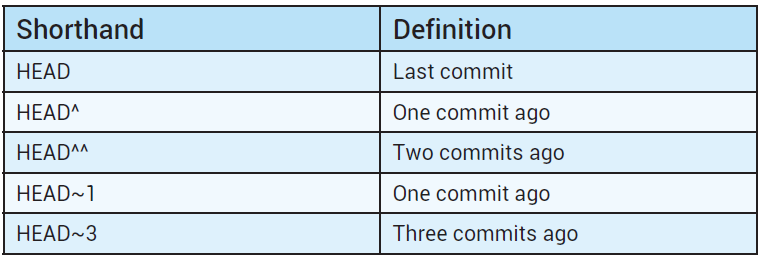
\includegraphics[width=0.9\textwidth]{figures/commitsShortHand}
\end{center}
{\small
You may use those short hands in all git command that may refer to a commit

\begin{shell}
\psone git log  HEAD-3..HEAD\\
\psone checkout HEAD^^
\end{shell}
The first command prints a log briefly describing the last 4 commits. The second position your working area to two commits ago.
\texttt{HEAD} may be thought as a pointer to the last commit.
}
\end{frame}
\begin{frame}{A graphical view}
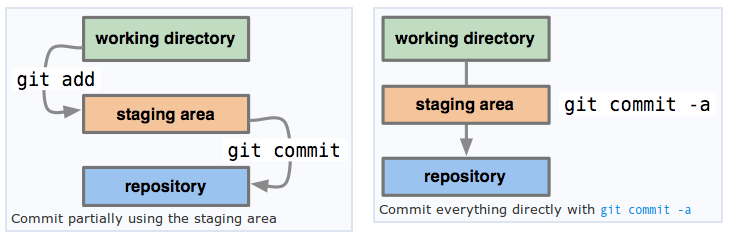
\includegraphics[width=\textwidth]{figures/commit}
\end{frame}

\begin{frame}{add, commit}
\titleline
So, the basic operations are
\begin{itemize}
\item \alert{git add file(s)} Add a snapshot of the file(s) to the staging area ready for commit. On a new file, it adds also the file to the git history.
\item \alert{git commit} Stores the staging area into the git local repository creating a new ``commit'' (also called blob).
\end{itemize}

\begin{shell}
\psone git commit -a
\end{shell}
commits all modified files.
\titleline
\end{frame}
\begin{frame}{Some advice}
\titleline
\begin{itemize}
\item Do atomic commits: each commit should be related to a single ``logical change'' in your code: a bug fix, a new feature... Avoid monster commits with a lot of files.

\item Write significant commit messages. Message like ``this is a commit'' are not allowed!

\item Git won't allow commits with empy messages.
\end{itemize}
\titleline
\end{frame}
\begin{frame}{Communicate with remote}
\titleline

To communicate with a remote repository we have three commands:
\alert{push}, \alert{fetch} and \alert{pull}.

We see now the simplest use of them. We assume we have a single remote
repository (\texttt{origin}) and a single branch (\texttt{master}).
\titleline
\end{frame}

\begin{frame}{Push}
\begin{shell}
git push
\end{shell}
Pushes all the commits for the current branch (\texttt{master} in this case)
onto the remote repo.
\end{frame}

\begin{frame}{Fetch}
\titleline
\begin{shell}
\psone git fetch
\end{shell}
Fetches all the commits for the current branch in the remote repository
and store them \alert{locally} in \texttt{remotes/origin/<branch>}

You can then examine them (read only!) by doing
\begin{shell}
\psone git checkout remotes/origin/new-branch
\end{shell}

You can finally merge the commits into your master
\begin{shell}
\psone git checkout master\\
\psone git merge remotes/origin/new_branch
\end{shell}
\titleline
\end{frame}
\begin{frame}{pull}
\begin{shell}
\psone git pull <branch>
\end{shell}

Is equivalent to \texttt{git fetch} followed by
\texttt{git merge}.

\alert{It is the most used command when you want to retrieve commits from a remote repository.}
\end{frame}

\begin{frame}{add, commit, push pull...}
\centerline{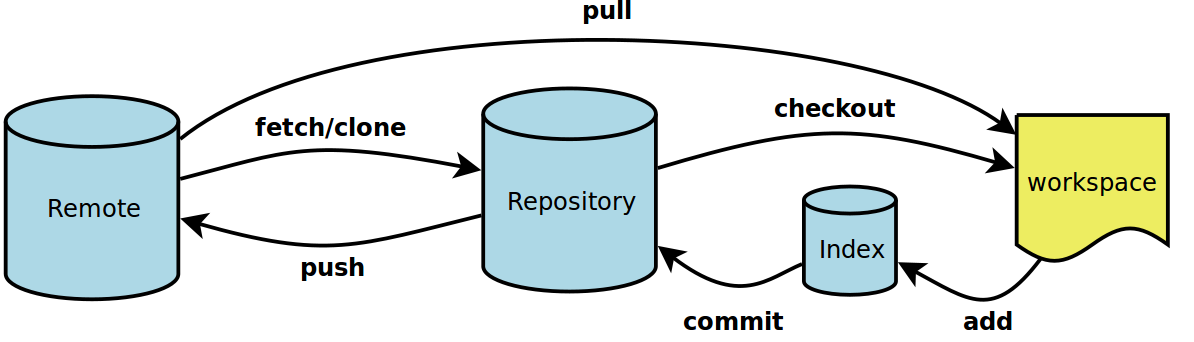
\includegraphics[width=\textwidth]{figures/pullandfetch}}
\end{frame}
\begin{frame}{git transport mechanism}
\centerline{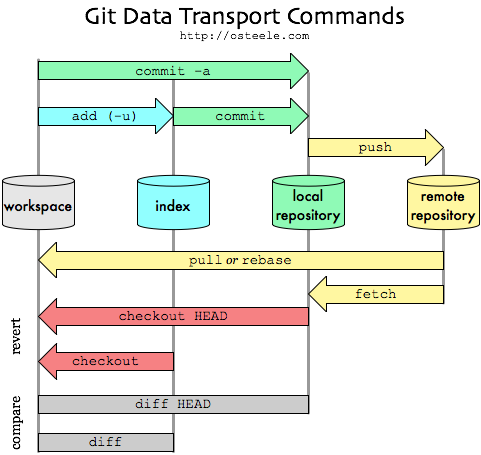
\includegraphics[width=0.8\textwidth]{figures/git-transport}}
\end{frame}

\begin{frame}{Merging gone wrong}
\begin{shell}
\psone git merge --abort
\end{shell}
cancels the merge.
\begin{shell}
\psone git diff <commit|branch>
\end{shell}
show differences between working tree and the commit (default HEAD).
\begin{shell}
\psone git mergetool <--tool=mytool>
\psone git mergetool --tool-help
\end{shell}
helps you in resolving conflict by using the tool you prefer. The second command gives you the list of tools.
\begin{shell}
\psone git difftool <--tool=mytool>
\end{shell}
Allows you to use a tool of choice for the diff.
\end{frame}

\begin{frame}{Branches}
\centerline{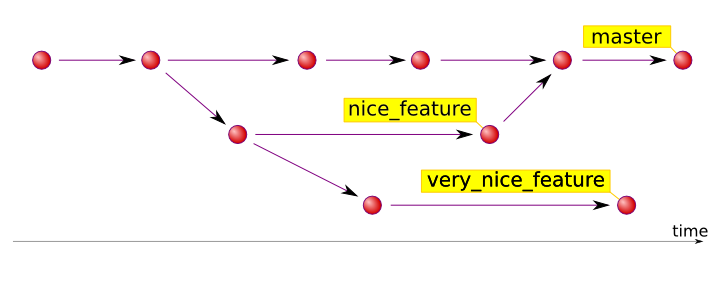
\includegraphics[width=0.7\textwidth]{figures/git-history}}

\titleline

Branches is one of the most important feature of git. When you create a repo you create also the \texttt{master} branch. But often you want to branch your tree to work on a specific topic without affecting the master branch.
\end{frame}
%%%%%%%%%%%%%%%%%%%%%%%%%%%%%%%%%%%%%%%%%%%%%%%%%
\begin{frame}{Branching- create}
create new branch
\begin{shell}
\psone git branch \var{shiny_new_branch} \\
\end{shell}
Go to that branch.
\begin{shell}
\psone git checkout \var{shiny_new_branch}
\end{shell}
Or create and position yourself in a new branch
\begin{shell}
\psone git checkout -b \var{shiny_new_branch}
\end{shell}

\end{frame}


\begin{frame}{Get other branches}
list local branches
\begin{shell}
\psone git branch \\
~ b1\\
* b2\\
~ master
\end{shell}
list remote branches (i.e. branches fetched from remote)
\begin{shell}
\psone git branch -r
\end{shell}
list all branches
\begin{shell}
\psone git branch -a
\end{shell}
LifeV branch name policy
\begin{shell}
YYYYMMDD_\var{meaningful_name}
\end{shell}
\end{frame}
%%%%%%%%%%%%%%%%%%%%%%%%%%%%%%%%%%%%%%%%%%%%%%%%%
\begin{frame}{Branching  - delete}
delete a branch
\begin{shell}
\psone git checkout master \\
\psone git branch -d \var{branch_to_delete}
\end{shell}
will cause an error if not merged with master!

To delete without merging
\begin{shell}
\psone git branch -D \var{branch_to_delete}
\end{shell}
delete a remote branch
\begin{shell}
\psone git push origin :\var{branch_to_delete}
\end{shell}
\begin{center}
\scriptsize%
the syntax comes from the generic generic push command\\
\tshell{git push \var{remotename} \var{localbranch_name}:\var{remotebranch_name}}\\
so we push an empty branch into the remote branch to be deleted
\end{center}
\end{frame}
%%%%%%%%%%%%%%%%%%%%%%%%%%%%%%%%%%%%%%%%%%%%%%%%%
\begin{frame}{Branching  - merge}
merge a branch
\begin{shell}
\psone git checkout master\\
\psone git merge \var{branch_name}\\
Updating e0f73f9..cd928c7\\
Fast-forward
\end{shell}
\pause
conflicts may arise!
\begin{shell}
CONFLICT (content): Merge conflict in file.cpp\\
Automatic merge failed; fix conflicts and then commit the result.
\end{shell}
\end{frame}
%%%%%%%%%%%%%%%%%%%%%%%%%%%%%%%%%%%%%%%%%%%%%%%%%
\begin{frame}[fragile]{Branching  - solve conflicts 1}
manual
\begin{shell}
\verb!<<<<<<<! HEAD\\
\ldots\\
=======\\
\ldots\\
\verb!>>>>>>>! branch_name\\
\end{shell}
\pause
text editor/gui
\begin{shell}
\psone git mergetool\\
merge tool candidates: meld opendiff kdiff3 tkdiff xxdiff tortoisemerge gvimdiff diffuse ecmerge p4merge araxis emerge vimdiff
\end{shell}
\end{frame}
%%%%%%%%%%%%%%%%%%%%%%%%%%%%%%%%%%%%%%%%%%%%%%%%%
\begin{frame}[fragile]{Branching  - solve conflicts 2}
after the diff are removed
\begin{shell}
\psone git add file.cpp
\end{shell}
a commit is needed when all the conflicts are solved!
\begin{shell}
\psone git commit
\end{shell}
\end{frame}
%
\begin{frame}{Merge tools}
If a merge has a commit, the command
\begin{shell}
\psone git mergetool --tool=<tool>
\end{shell}

opens a graphical interface to handle conflicts.
\end{frame}

  
\begin{frame}{Branching  - stash}
checkout with hanging modifications is forbidden!
\begin{shell}
\psone git checkout master\\
error: Your local changes to the following files would be overwritten by checkout: \ldots
\end{shell}
we can stash modifications
\begin{shell}
\psone git stash save
\end{shell}
and bring them back
\begin{shell}
\psone git stash \{ pop | apply \}
\end{shell}
remember to clear the stash (in particular if you use apply).
\begin{shell}
\psone git stash list\\
\psone git stash clear
\end{shell}
\end{frame}
%%%%%%%%%%%%%%%%%%%%%%%%%%%%%%%%%%%%%%%%%%%%%%%%%%
\begin{frame}{Merging and rebasing}
There are two ways in git to integrate work from one branch to the other.
\begin{center}
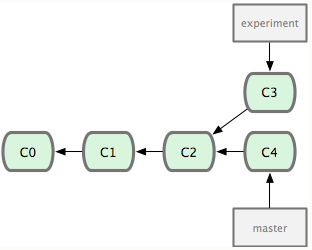
\includegraphics[width=0.7\textwidth]{figures/tomerge}
\end{center}
\end{frame}
\begin{frame}{Merge}
\begin{shell}
\psone git checkout master\\
\psone git merge experiment
\end{shell}
\begin{center}
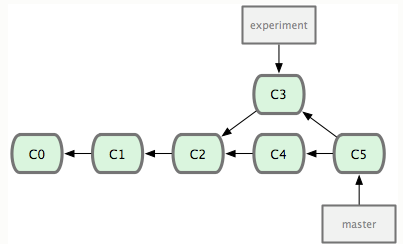
\includegraphics[width=0.7\textwidth]{figures/merged}
\end{center}
\end{frame}
\begin{frame}{Rebase}
\begin{shell}
\psone git checkout experiment\\
\psone git rebase master
\end{shell}
\begin{center}
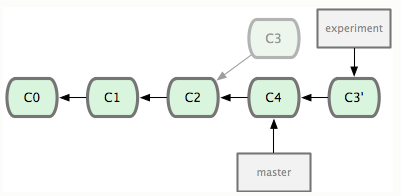
\includegraphics[width=0.8\textwidth]{figures/rebase1}
\end{center}
\end{frame}
\begin{frame}{A merge to realign master with experiment}
\begin{shell}
\psone git checkout master\\
\psone git merge experiment
\end{shell}
\begin{center}
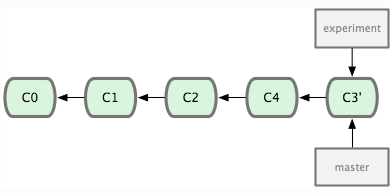
\includegraphics[width=0.8\textwidth]{figures/rebase2}\\
\end{center}
\end{frame}
\begin{frame}{Rebase (alternative form)}
\begin{shell}
\psone git rebase master experiment\\
\end{shell}
\begin{center}
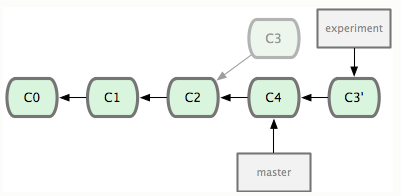
\includegraphics[width=0.8\textwidth]{figures/rebase1}\\
\end{center}
\end{frame}

\begin{frame}{The differences}
Merge does a three way merge. The history after the merge reflects what has happened. You create a commit with \alert{2 parents}.
\medskip

Rebase ``replays'' commits on the base on top of another branch. It will produce a \alert{linear history}, easier to read.

Rebasing is also more general: you can select the commits to rebase (advanced topic).
\end{frame}

\begin{frame}{When merging? When rebasing?}
Rebase is useful if one wants to keep a linear history. It could be the method of choice to merge on an important branch work done on a \alert{only local} topic branch.

\textcolor{blue}{Rebase however rewrites history changing commits.} So 
\alert{it should never rebase using shared branches, where several developers are working.}
\end{frame}

%%%%%%%%%%%%%%%%%%%%%%%%%%%%%%%%%%%%%%%%%%%%%%%%%
\begin{frame}{Collaboration - remote}
share a branch with a remote repo
\begin{shell}
\psone git push \var{repo_name} \var{branch_name}\\
\psone git pull \var{repo_name} \var{branch_name}
\end{shell}
setup remote link
\begin{shell}
\psone git config branch.\var{branch_name}.remote \nl \var{repo_name}\\
\psone git config branch.\var{branch_name}.merge \nl refs/heads/\var{branch_name}
\end{shell}
the others can access the branch with
\begin{shell}
\psone[alessio] git checkout \var{branch_name}
\psone[nur] git checkout -{}-track -b \var{branch_name} \nl \var{repo_name}/\var{branch_name}
\end{shell}
\end{frame}
%%%%%%%%%%%%%%%%%%%%%%%%%%%%%%%%%%%%%%%%%%%%%%%%%
\begin{frame}{Collaboration - local}
share a branch locally
\begin{shell}
\psone[nur] git remote add ant_repo \nl /path/to/ant/git/repo\\
\psone[nur] git fetch ant_repo\\
\psone[nur] git checkout -{}-track -b shared_branch \nl ant_repo/my_super_secret_branch
\end{shell}
push modifications to the original branch
\begin{shell}
\psone[nur] git checkout shared_branch\\
\psone[nur] git push ant_repo shared_branch
\end{shell}
or pull them from the original repo
\begin{shell}
\psone git remote add nur_repo /path/to/nur/git/repo\\
\psone git fetch nur_repo /path/to/nur/git/repo\\
\psone git checkout my_super_secret_branch\\
\psone git pull nur_repo/shared_branch
\end{shell}
check for read/write permissions!
\end{frame}
%%%%%%%%%%%%%%%%%%%%%%%%%%%%%%%%%%%%%%%%%%%%%%%%
\begin{frame}{Fixing commits: amend reset and revert}
Sometimes you want to correct your \alert{last commit}
\begin{shell}
\psone <do your additional work/add/rm>\\
\psone git commit --amend
\end{shell}
\smallskip

\alert{Never amend a commit that has been already pushed: use git revert}
\end{frame}

\begin{frame}{Reset}
\texttt{git reset} sets yours HEAD to a specified commit. So it can be used to ``delete commits'' 
{\small
\begin{shell}
\psone git reset <file>
\end{shell}
Removes the specified file from the staging area, but leave the working directory unchanged. This unstages a file without overwriting any changes.
It is the opposite of \texttt{git add}.

\begin{shell}
\psone git reset
\end{shell}
This unstages all files without overwriting any changes, giving you the opportunity to re-build the staged snapshot from scratch.
\begin{shell}
\psone git reset <commit>
\end{shell}
Move the current branch tip backward to <commit>, reset the staging area to match, but leave the working directory alone. All changes made since <commit> will reside in the working directory.
}
\end{frame}

\begin{frame}{Hard Reset}
\begin{shell}
\psone git reset --hard
\end{shell}
{\small 
In addition to unstaging changes, the --hard flag tells Git to \alert{overwrite all changes in the working directory} too. Put another way: \alert{this obliterates all uncommitted changes}, so make sure you really want to throw away your local developments.
}
\begin{shell}
\psone git reset --hard <commit>
\end{shell}
{\small Move the current branch tip backward to <commit> and reset both the staging area and the working directory to match. This obliterates not only the uncommitted changes, but all commits after <commit>, as well.
}
\begin{shell}
\psone git reset [--|<commit>] [--hard] <paths>
\end{shell}
{
\small
resets all index entries of <paths> to their state at \texttt{commit}.
}
\end{frame}

\begin{frame}{A warning}
Reset may change the history. \alert{Do not use it on commits to ``delete'' that have already been pushed to the repository}.
\end{frame}
\begin{frame}{Revert}
\texttt{git revert} reverts commits by \alert{playing them backwards}. So it does not ``delete'' them. It is history safe.
\begin{shell}
\psone git revert HEAD\textasciitilde{}3
\end{shell}

reverts the changes specified by the fourth last commit in HEAD and
          create a new commit with the reverted changes.
\smallskip

\alert{It requires your working tree to be clean.}
\end{frame}

\begin{frame}{Get info}
\begin{shell}
\psone git log
\end{shell}
Shows commit logs.
\begin{shell}
\psone git shortlog
\end{shell}
Summarizes log output, showing commit description from each contributor 
\begin{shell}
\psone git show <object>
\end{shell}
Show some properties of the \texttt{object} (blob, commit...). 
\alert{Use a graphical interface like \texttt{gitk}...}
\end{frame}
%%%%%%%%%%%%%%%%%%%%%%%%%%%%%%%%%%%%%%%%%%%%%%%%% 
\begin{frame}{Common issues - I}
\boxltr{Q} edited on master branch by mistake, I wanted to do in new\_branch instead!
\pause

\boxltr{A} a simple checkout will do it
\begin{shell}
\psone git checkout -b new_branch
\end{shell}
\pause
\boxltr{Q} already committed to master branch
\pause

\boxltr{A} create a new branch and delete the commit on master
\begin{shell}
\psone git branch new_branch\\
\psone git reset -{}-hard HEAD\textasciitilde1\\
\psone git checkout new_branch\\
\end{shell}
\end{frame}

%%%%%%%%%%%%%%%%%%%%%%%%%%%%%%%%%%%%%%%%%%%%%%%%% 
\begin{frame}{Common issues - II}
\boxltr{Q} I want to discard my edit and get the latest version of the file!
\pause

\boxltr{A} Simple
\begin{shell}
\psone git checkout -- file
\end{shell}
\pause
\boxltr{Q} I want to get the file from another branch or another commit!
\pause

\boxltr{A} It's the same command as before:
\begin{shell}
\psone git checkout <branch|commit> -- file
\end{shell}
\end{frame}

%%%%%%%%%%%%%%%%%%%%%%%%%%%%%%%%%%%%%%%%%%%%%%%%%
\begin{frame}{Common issues - II}
\boxltr{Q} Get a from another branch
\pause

\boxltr{A} cherry-pick it to the correct one
\begin{shell}
\psone git checkout correct_branch\\
\psone git cherry-pick commit_hash
\end{shell}
\pause

\boxltr{Q} cannot get the branch of the local remote
\pause

\boxltr{A} missing references to the other branches
\begin{shell}
\psone git fetch remote_name\\
\psone git remote show remote_name
\end{shell}
\end{frame}
%%%%%%%%%%%%%%%%%%%%%%%%%%%%%%%%%%%%%%%%%%%%%%%%%
\begin{frame}{Common issues - III}
\boxltr{Q} the merge has gone bananas!
\pause

\boxltr{A} give up the merge and try again
\begin{shell}
\psone git merge \var{branch_to_be_merged}\\
\psone \#\$!\&\#\%\$\@\&\^\@ \\
\psone git reset -{}-hard \var{original_branch}
\end{shell}
\pause
or, more simply
\begin{shell}
git merge --abort
\end{shell}

\boxltr{Q} i want a file from that branch!
\pause

\boxltr{A} get it with
\begin{shell}
\psone git checkout \var{branch} \var{files}\\
\end{shell}
\end{frame}
%%%%%%%%%%%%%%%%%%%%%%%%%%%%%%%%%%%%%%%%%%%%%%%%%
\begin{frame}{Common issues - IV}
\boxltr{Q} git push refuses to work

\begin{shell}
\tiny
remote: error: refusing to update checked out branch: refs/heads/\var{branch_name}\\
remote: error: By default, updating the current branch in a non-bare repository\\
remote: error: is denied, because it will make the index and work tree inconsistent\\
remote: error: with what you pushed, and will require 'git reset --hard' to match\\
remote: error: the work tree to HEAD.\\
remote: error:\\
remote: error: You can set 'receive.denyCurrentBranch' configuration variable to\\
remote: error: 'ignore' or 'warn' in the remote repository to allow pushing into\\
remote: error: its current branch; however, this is not recommended unless you\\
remote: error: arranged to update its work tree to match what you pushed in some\\
remote: error: other way.\\
remote: error:\\
remote: error: To squelch this message and still keep the default behaviour, set\\
remote: error: 'receive.denyCurrentBranch' configuration variable to 'refuse'.\\
To \var{repo}\\
 ! [remote rejected] \var{branch_name} -> \var{branch_name} (branch is currently checked out)\\
\end{shell}

\pause

\boxltr{A} use a bare repo
\begin{shell}
\psone git clone --bare \var{repo} \var{repo}.git\\
\end{shell}
\begin{center}
\tiny\url{http://stackoverflow.com/questions/2199897/git-convert-normal-to-bare-repository}
\end{center}
\end{frame}
%%%%%%%%%%%%%%%%%%%%%%%%%%%%%%%%%%%%%%%%%%%%%%%%%
\begin{frame}[fragile]{Tips \& tricks - I}
\begin{itemize}[<+->]
\item \tshell{gitk} is your friend
\item do small, atomic commits
\item read git output
\item branch in \tshell{PS1}: add to \texttt{.bashrc}
\begin{shell}
\tiny
function GitBranch \{\\
~~\verb!_branch="$(git branch 2>/dev/null | sed -e "/^\s/d"!\\
~~\verb!-e "s/^\*\s//")"!\\
~~\verb!test -n "$_branch" && echo -e "@$_branch"!\\
\}\\
PS1=\textquotesingle\verb!\u@\h:\w$(GitBranch)> !\textquotesingle
\end{shell}
\vspace*{0.25cm}
\item watch out for non history-safe commands after pushing!
{\footnotesize(\tshell{cherry-pick},\tshell{rebase},\ldots)}
\item everything else (and more\ldots) on git
\begin{center}
\url{http://book.git-scm.com/index.html}
\end{center}
\end{itemize}
\end{frame}
%%%%%%%%%%%%%%%%%%%%%%%%%%%%%%%%%%%%%%%%%%%%%%%%%
\begin{frame}{Tips \& tricks - II}
\begin{itemize}[<+->]
\item bash autocompletion
\begin{center}
\footnotesize
\url{http://git.kernel.org/?p=git/git.git;a=blob_plain;f=contrib/completion/git-completion.bash;hb=HEAD}
\end{center}
\item colored output
\begin{shell}
\psone git config -{}-global color.ui true
\end{shell}
\vspace*{0.25cm}
\item no empty push
\begin{shell}
\psone git config -{}-global push.default nothing
\end{shell}
\vspace*{0.25cm}
\item creating archives
\begin{shell}
\psone git archive \var{commit_or_branch} | gzip > \nl \var{archive_name}.tgz
\end{shell}
\end{itemize}
\end{frame}
%%%%%%%%%%%%%%%%%%%%%%%%%%%%%%%%%%%%%%%%%%%%%%%%%
\end{document}
